\documentclass[12pt]{article}

\usepackage[utf8]{inputenc}
\usepackage[T1]{fontenc}
\usepackage[spanish,es-noshorthands]{babel}
\usepackage{newtxtext,newtxmath}      % Times New Roman + matematicas
\usepackage[a4paper,margin=2.5cm]{geometry}
\usepackage{graphicx}
\graphicspath{{figuras/}{../resultados/graficas/}}
\usepackage{booktabs}
\usepackage{array}
\usepackage{tabularx}
\usepackage{amsmath,amssymb}
\usepackage{xcolor}
\usepackage{float}
\usepackage{caption}
\usepackage{subcaption}
\usepackage{enumitem}
\usepackage{listings}
\usepackage[hidelinks]{hyperref}

\captionsetup{font=small, labelfont=bf}
\setlength{\parskip}{0.25\baselineskip}
\linespread{1.0}                       % interlineado sencillo

\lstdefinestyle{cod}{
  basicstyle=\ttfamily\footnotesize, breaklines=true, columns=fullflexible,
  keepspaces=true, frame=single, framesep=4pt, rulecolor=\color{gray},
  showstringspaces=false, backgroundcolor=\color{gray!8}, xleftmargin=6pt}
\lstset{style=cod}

% ============================================================================
\begin{document}

% ------------------------------- Portada ------------------------------------
\begin{center}
  {\LARGE\bfseries Benchmarking de código C++ paralelo generado por IA:\\[2pt]
   estudio comparativo de rendimiento en convolución de imágenes con OpenMP\par}
  \vspace{6pt}
  {\large Benchmarking of AI-generated parallel C++ code: a comparative\\
   performance study of image convolution with OpenMP\par}
\end{center}

\vspace{4pt}
\begin{center}
  \textbf{Jose Barrera Ramos}, \textbf{Miguel Padilla}, \textbf{Esteban Serrano}\\[2pt]
  {\small Pontificia Universidad Javeriana Cali, Facultad de Ingeniería,\\
   Santiago de Cali, Colombia.}
\end{center}

\vspace{6pt}
\hrule
\vspace{8pt}

% ------------------------------- Resumen ------------------------------------
\noindent\textbf{Resumen}
\vspace{2pt}

\noindent\textbf{Objetivo:} determinar el impacto de la paralelización sobre el
rendimiento de código C++ generado por IA en convolución 2D, frente a una línea
base secuencial, una variante IA optimizada y una implementación manual.
\textbf{Materiales y métodos:} cuatro variantes (secuencial, paralelo IA, IA
optimizado y manual, con OpenMP) comparten kernel gaussiano, borde replicado y
validación de equivalencia estricta (checksum FNV-1a de 64 bits). Se evaluaron
imágenes de 512, 1024, 2048 y 4096 px de lado, kernels de 3, 5, 7 y 11, y 1, 2, 4,
8 y 16 hilos, con 30 ejecuciones cronometradas por configuración, midiendo solo el
tiempo de convolución.
\textbf{Resultados y discusión:} la paralelización redujo el tiempo hasta
$7.98\times$ (imagen 2048, kernel 3, 16 hilos); IA optimizado superó a IA en
24.6\,\% en promedio a un hilo (hasta 34.2\,\%); los checksums coincidieron en
48/48 configuraciones (0 fallos).
\textbf{Conclusiones:} el código generado por IA fue competitivo con el manual
($5.58\times$ y $5.07\times$ a 16 hilos en 4096); la optimización posterior elevó
el speedup a $7.35\times$ (kernel 11).

\vspace{10pt}
\hrule

% ------------------------------- Abstract -----------------------------------
\noindent\textbf{Abstract}
\vspace{2pt}

\noindent\textbf{Objective:} to determine the impact of parallelization on the
performance of AI-generated C++ code for 2D convolution, against a sequential
baseline, an optimized AI variant, and a hand-written implementation.
\textbf{Materials and methods:} four variants (sequential, AI, optimized AI, and
hand-written, with OpenMP) share a Gaussian kernel, replicated borders, and a
strict equivalence check (64-bit FNV-1a checksum). Images of 512, 1024, 2048 and
4096 px per side, kernels of 3, 5, 7 and 11, and 1, 2, 4, 8 and 16 threads were
evaluated, with 30 timed runs per configuration, measuring only the convolution
time.
\textbf{Results and discussion:} parallelization reduced the time by up to
$7.98\times$ (2048 image, kernel 3, 16 threads); optimized AI improved on AI by
24.6\,\% on average at one thread (up to 34.2\,\%); checksums matched in 48/48
configurations (0 failures).
\textbf{Conclusions:} the AI-generated code was competitive with the hand-written
one ($5.58\times$ and $5.07\times$ at 16 threads on 4096); the subsequent
optimization raised the speedup to $7.35\times$ (kernel 11).

\vspace{10pt}
\hrule

% ============================================================================
\section{Introducción}
\label{sec:intro}

La generación automática de código asistida por modelos de lenguaje (IA) se ha
convertido en una herramienta habitual de programación. Una pregunta abierta es
si el código paralelo producido por IA es competitivo, en términos de rendimiento,
frente al código escrito por una persona. Responderla exige una comparación
controlada: mismas entradas, mismos parámetros y mismo hardware y software.

Este trabajo estudia el caso de una \textbf{convolución 2D} de imágenes, un
núcleo computacionalmente intensivo y altamente paralelizable, aplicada con un
\textbf{filtro gaussiano}. El objetivo general es \emph{determinar el impacto de
la paralelización sobre el rendimiento del código C++ generado mediante IA}
mediante pruebas controladas bajo idénticas condiciones de hardware, software,
imágenes de entrada y parámetros de convolución.

Las contribuciones de este artículo son:
\begin{itemize}[leftmargin=1.4em,itemsep=1pt]
  \item un \textbf{diseño experimental reproducible} (contenedor Docker) que
        compara cuatro variantes de un mismo algoritmo;
  \item una \textbf{validación de equivalencia estricta} (bit a bit) basada en un
        checksum de 64 bits, que garantiza que las diferencias de tiempo no se
        deben a resultados distintos;
  \item un \textbf{análisis cuantitativo} de tiempo, speedup y eficiencia en
        función del tamaño de imagen, del tamaño de kernel y del número de hilos;
  \item una comparación entre código \textbf{secuencial}, \textbf{paralelo IA},
        \textbf{IA~+~optimizado} y \textbf{manual}.
\end{itemize}

El resto del artículo se organiza así: la Sección~\ref{sec:metodos} describe los
materiales y métodos; la Sección~\ref{sec:resultados} presenta los resultados y su
discusión; la Sección~\ref{sec:conclusiones} resume las conclusiones. El Anexo
documenta la reproducibilidad del experimento.

\paragraph{Alcance.} El estudio se limita a una carga (convolución 2D con kernel
gaussiano), a un único lenguaje (C++ con OpenMP) y a un único equipo de cómputo.
Los resultados deben interpretarse dentro de ese alcance.

% ============================================================================
\section{Materiales y métodos}
\label{sec:metodos}

\subsection{Objetivo e hipótesis}
\label{subsec:objetivo}
El objetivo específico es cuantificar el \textbf{speedup} y la \textbf{eficiencia}
de cada variante paralela respecto de la secuencial, y evaluar la
\textbf{competitividad técnica} del código generado por IA frente a una versión
manual. Las hipótesis de trabajo son:
\begin{description}[leftmargin=1.4em,itemsep=1pt]
  \item[H1.] El código paralelo generado por IA alcanza un speedup cercano al de
  la implementación manual, porque ambas paralelizan el mismo algoritmo de la
  misma forma (un bucle \texttt{for} paralelo sobre las filas).
  \item[H2.] La variante IA~+~optimizada supera a la IA base incluso a un solo
  hilo, porque su ventaja proviene de optimizaciones de memoria y vectorización,
  no de paralelizar mejor.
  \item[H3.] La eficiencia decrece al aumentar el número de hilos, por
  \emph{overhead} de sincronización, contención de memoria y heterogeneidad de
  núcleos (ley de Amdahl).
\end{description}

\subsection{Imágenes de entrada y kernels}
\label{subsec:datos}
Se emplea un único conjunto de cuatro imágenes de entrada de $512\times512$,
$1024\times1024$, $2048\times2048$ y $4096\times4096$ px; todas se normalizan a
\textbf{RGB (3 canales)} antes de convolucionar. El filtro es un \textbf{kernel
gaussiano normalizado} (suma = 1) de tamaño $3\times3$, $5\times5$, $7\times7$ y
$11\times11$, con
\begin{equation}
  \sigma = 0.3\left(\frac{K-1}{2}-1\right) + 0.8 ,
  \label{eq:sigma}
\end{equation}
donde $K$ es el lado del kernel. El borde se resuelve por
\textbf{replicación} (\emph{clamp}), de modo que la salida conserva el tamaño de
la entrada. Estas definiciones se fijan en código y son idénticas en las cuatro
variantes.

\subsection{Variantes C++ comparadas}
\label{subsec:variantes}
Las cuatro variantes calculan exactamente la misma operación y producen la misma
imagen; solo cambia cómo está escrito el código (Tabla~\ref{tab:variantes}).

\begin{table}[H]
\centering
\caption{Variantes C++ comparadas.}
\label{tab:variantes}
\small
\begin{tabularx}{\linewidth}{@{}l l l X@{}}
\toprule
\textbf{Variante} & \textbf{Paralelismo} & \textbf{Origen} & \textbf{Descripción} \\
\midrule
Secuencial & --- & Manual & Línea base a 1 hilo; referencia $T_1$ y checksum patrón. \\
Paralelo IA & OpenMP & Generada por IA & Bucle \texttt{parallel for} sobre las filas. \\
Paralelo IA~+~Opt. & OpenMP & IA + ajuste manual & Inversión de bucles (SIMD) y fusión de canales RGB. \\
Paralelo Manual & OpenMP & 100\,\% a mano & Adaptada del repositorio de GitHub \cite{githubconv}. \\
\bottomrule
\end{tabularx}
\end{table}

\paragraph{Secuencial.} Para cada píxel $(y,x)$ y canal $c$ acumula la suma
ponderada de sus vecinos en \texttt{float}, con el orden (primero $k_y$, luego
$k_x$) de la Ec.~\ref{eq:conv}:
\begin{equation}
  \mathrm{out}(y,x,c)=\mathrm{clamp}\!\Big(\mathrm{round}\!\sum_{k_y=-r}^{r}\sum_{k_x=-r}^{r}
  K(k_y,k_x)\,I(y+k_y,\,x+k_x,\,c)\Big),\quad r=\lfloor K/2\rfloor .
  \label{eq:conv}
\end{equation}

\paragraph{Paralelo IA.} Idéntico al secuencial, pero distribuye las filas entre
los hilos:
\begin{lstlisting}
#pragma omp parallel for schedule(static)
for (int y = 0; y < h; ++y) { /* convolucion de la fila y */ }
\end{lstlisting}
Cada hilo escribe filas distintas; no hay condiciones de carrera.

\paragraph{Paralelo IA~+~opt.} Aplica dos optimizaciones que preservan el
resultado: (i)~\textbf{inversión de bucles}, de modo que el bucle más interno
recorre una fila completa con un acumulador por píxel (vectorizable con SIMD); y
(ii)~\textbf{fusión de canales RGB}, leyendo cada píxel de entrada una sola vez en
lugar de tres. La suma por píxel y canal conserva el orden $(k_y,k_x)$, por lo que
el resultado es idéntico bit a bit.

\paragraph{Paralelo manual.} Se adaptó un código humano de convolución
disponible en GitHub \cite{githubconv}, conservando su esencia (una función
\texttt{kernel\_calc} por píxel, una función \texttt{convolution} con
\texttt{parallel for} y \texttt{schedule(static, 2)}, y \texttt{applyFilter} por
canal), pero ajustándolo a tamaño y kernel dinámicos, borde replicado y
acumulación en \texttt{float}.

\subsection{Equivalencia estricta y validación}
\label{subsec:validacion}
Para que la comparación de tiempos sea válida, todas las variantes deben producir
\textbf{el mismo resultado}. Por ello, cada programa calcula un \textbf{checksum
FNV-1a de 64 bits} sobre el búfer RGB de salida, que debe ser idéntico al de la
versión secuencial, para cada imagen y kernel, y constante entre los distintos
números de hilos. Para preservar la equivalencia bit a bit, todas las variantes se
compilan con la misma optimización y con \texttt{-ffp-contract=off} (sin
contracción a FMA) y usan el mismo tipo (\texttt{float}) y el mismo orden de
operaciones.

\subsection{Hardware y software}
\label{subsec:entorno}
La Tabla~\ref{tab:entorno} resume el entorno experimental. La ejecución se realiza
íntegramente dentro de un contenedor \textbf{Docker} para garantizar
reproducibilidad entre equipos.

\begin{table}[H]
\centering
\caption{Entorno experimental.}
\label{tab:entorno}
\small
\begin{tabularx}{\linewidth}{@{}l X@{}}
\toprule
\textbf{Elemento} & \textbf{Descripción} \\
\midrule
CPU & Intel Core i5-12450HX (12.\textsuperscript{a} gen), 8 núcleos (4 P + 4 E), 12 hilos lógicos, 2.4 GHz base \\
Memoria RAM & 24 GB \\
Núcleos visibles por el contenedor & 12 \\
Sistema operativo anfitrión & Windows 11 Home (64 bits) \\
Contenedor & Ubuntu 24.04, compilación con \texttt{g++}/CMake, \texttt{-O2}, OpenMP \\
Docker & Docker Desktop (cliente 29.6.2) y Compose v5.3.1 \\
Política de compilación & \texttt{-O2}, \texttt{-ffp-contract=off}, sin \emph{fast-math} \\
\bottomrule
\end{tabularx}
\end{table}

\subsection{Protocolo experimental}
\label{subsec:protocolo}
Para cada combinación (imagen, kernel, hilos) y cada variante se realizan
\textbf{30 ejecuciones cronometradas} precedidas de \textbf{1 ejecución de
calentamiento} no cronometrada. Se cronometra \textbf{únicamente el bucle de
convolución}; la carga y el guardado de la imagen quedan fuera de la medición. Los
hilos evaluados en las variantes paralelas son \textbf{1, 2, 4, 8 y 16}; la versión
secuencial siempre corre con 1. El número de repeticiones y la carpeta de imágenes
son parámetros de entorno (\texttt{BENCH\_REPS}, \texttt{BENCH\_DATASET}), sin
recompilar.

\subsection{Métricas}
\label{subsec:metricas}
Para cada configuración se registra el tiempo de convolución en milisegundos y se
calculan la media $\mu$, la desviación estándar muestral $s$ (con $n-1$ grados de
libertad), el mínimo y el máximo de las 30 mediciones (Ec.~\ref{eq:stats}):
\begin{equation}
  \mu=\frac{1}{n}\sum_{i=1}^{n} t_i, \qquad
  s=\sqrt{\frac{1}{n-1}\sum_{i=1}^{n}(t_i-\mu)^2}.
  \label{eq:stats}
\end{equation}
Además, para cada programa y configuración se calculan el \textbf{speedup} y la
\textbf{eficiencia}:
\begin{equation}
  S(p)=\frac{T_1}{T_p}, \qquad E(p)=\frac{S(p)}{p},
  \label{eq:speedup}
\end{equation}
donde $T_1$ es el tiempo de la versión secuencial y $T_p$ el de la variante
paralela con $p$ hilos (misma imagen y mismo kernel).

\subsection{Reproducibilidad}
\label{subsec:repro}
El proyecto se distribuye con un \texttt{Dockerfile}, un \texttt{docker-compose.yml}
y scripts que automatizan la corrida y la evaluación (generación de un CSV único,
tablas Markdown y gráficas). La lectura y escritura de imágenes usa la librería
\texttt{stb} \cite{stb}. Los comandos exactos se documentan en el
Anexo~\ref{anexo:repro}. La seed no aplica (no hay aleatoriedad en el cómputo); el
conjunto de imágenes es fijo y versionado.

% ============================================================================
\section{Resultados y discusión}
\label{sec:resultados}

\subsection{Validación de equivalencia estricta}
Las 48 configuraciones (variante, imagen, kernel) de las tres variantes paralelas
produjeron un checksum idéntico al de la versión secuencial, en todos los números
de hilos y a lo largo de las 30 repeticiones: \textbf{48/48 coinciden, 0 fallos}
(Tabla~\ref{tab:validacion}). Esto confirma que las diferencias de tiempo se deben
al rendimiento y no a resultados distintos, y habilita la comparación de speedup.

\begin{table}[H]
\centering
\caption{Validación de equivalencia estricta (checksum FNV-1a).}
\label{tab:validacion}
\small
\begin{tabular}{@{}lccc@{}}
\toprule
\textbf{Variante} & \textbf{Config. (imagen$\times$kernel)} & \textbf{Coinciden} & \textbf{Fallos} \\
\midrule
Paralelo IA        & 16 & 16 & 0 \\
Paralelo IA~+~Opt  & 16 & 16 & 0 \\
Paralelo Manual    & 16 & 16 & 0 \\
\midrule
\textbf{Total}     & \textbf{48} & \textbf{48} & \textbf{0} \\
\bottomrule
\end{tabular}
\end{table}

\subsection{Tiempo de ejecución}
La Tabla~\ref{tab:secuencial} presenta la línea base secuencial: el tiempo crece
de forma aproximadamente lineal con el número de píxeles y de forma cuadrática con
el lado del kernel. La imagen $4096\times4096$ con kernel $11\times11$ es el caso
más costoso (5664 ms).

\begin{table}[H]
\centering
\caption{Tiempo medio de convolución de la versión secuencial (ms), 30 repeticiones.}
\label{tab:secuencial}
\small
\begin{tabular}{@{}lrrrr@{}}
\toprule
\textbf{Imagen} & \textbf{3$\times$3} & \textbf{5$\times$5} & \textbf{7$\times$7} & \textbf{11$\times$11} \\
\midrule
$512\times512$     &    9.56 &   22.72 &   37.89 &    92.40 \\
$1024\times1024$   &   38.10 &   82.22 &  154.30 &   356.43 \\
$2048\times2048$   &  164.06 &  313.82 &  568.22 &  1368.71 \\
$4096\times4096$   &  608.32 & 1305.55 & 2367.26 &  5664.25 \\
\bottomrule
\end{tabular}
\end{table}

La Tabla~\ref{tab:tiempo} muestra el tiempo absoluto para el caso más costoso
($4096\times4096$, kernel $11\times11$). Todas las variantes paralelas reducen el
tiempo de forma monótona con los hilos; el mejor tiempo lo alcanza IA~+~Opt con
16 hilos (771 ms, frente a 5664 ms de la secuencial). La Fig.~\ref{fig:tiempo_cmp}
compara directamente las variantes y la Fig.~\ref{fig:tiempo_ia} desglosa el
comportamiento por imagen y kernel.

\begin{table}[H]
\centering
\caption{Tiempo medio de convolución (ms), imagen $4096\times4096$, kernel $11\times11$.}
\label{tab:tiempo}
\small
\begin{tabular}{@{}lrrrrr@{}}
\toprule
\textbf{Variante} & \textbf{1 h} & \textbf{2 h} & \textbf{4 h} & \textbf{8 h} & \textbf{16 h} \\
\midrule
Secuencial         & 5664.2 &   --- &   --- &   --- &   --- \\
Paralelo IA        & 5422.4 & 2764.7 & 1647.4 & 1126.2 &  978.0 \\
Paralelo IA~+~Opt  & 4296.8 & 2250.9 & 1321.8 &  908.7 &  771.1 \\
Paralelo Manual    & 5709.5 & 2921.8 & 1877.3 & 1372.7 & 1144.0 \\
\bottomrule
\end{tabular}
\end{table}

\begin{figure}[H]\centering
  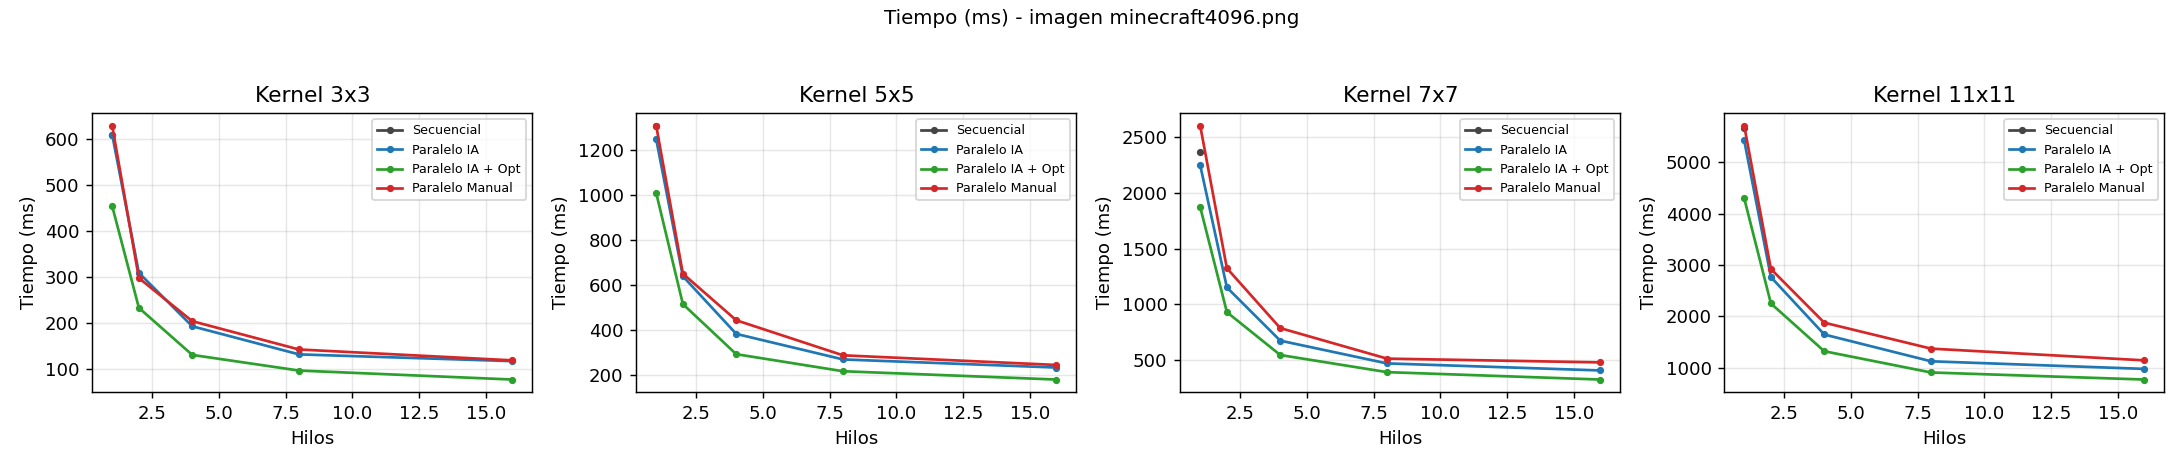
\includegraphics[width=0.9\linewidth]{comparacion_tiempo.png}
  \caption{Tiempo de convolución (ms) vs.\ número de hilos: comparación directa
  entre variantes sobre la imagen más grande.}
  \label{fig:tiempo_cmp}
\end{figure}

\begin{figure}[H]\centering
  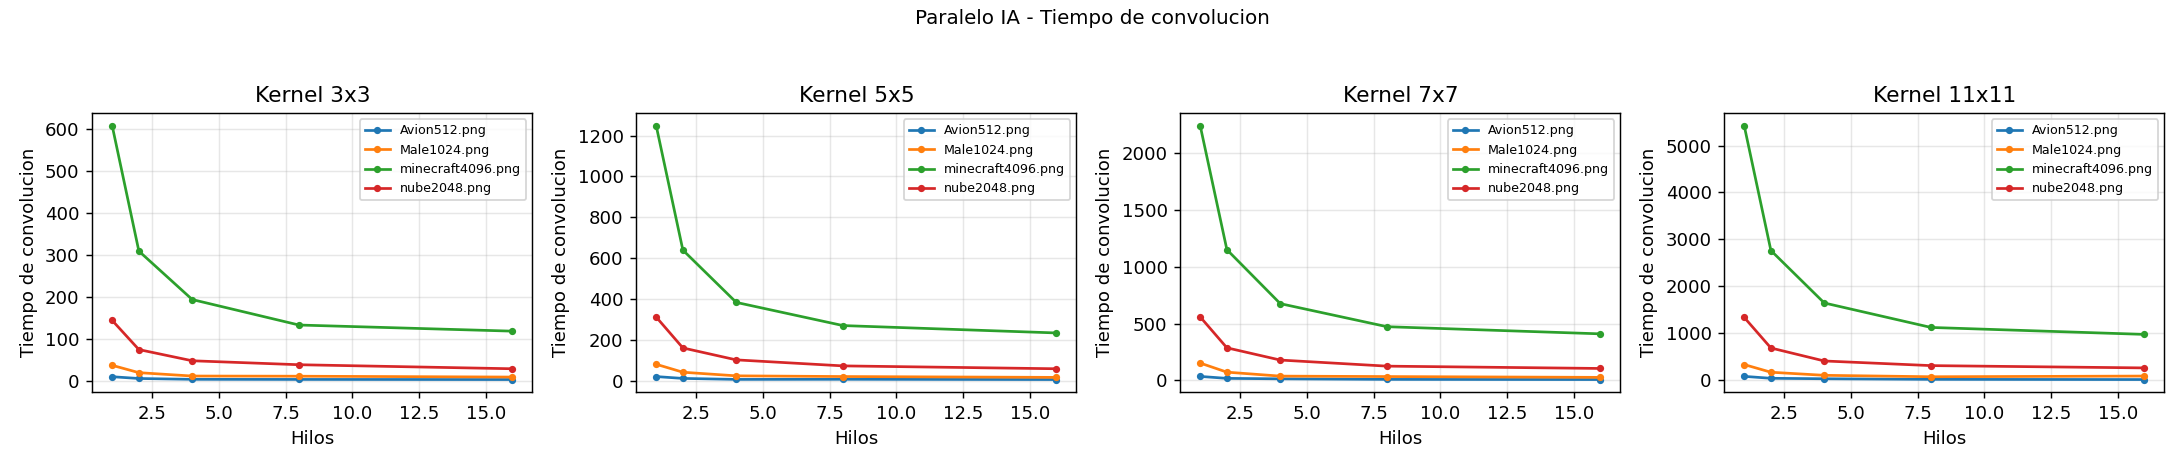
\includegraphics[width=0.9\linewidth]{tiempo_paralelo_ia.png}
  \caption{Tiempo de convolución (ms) vs.\ número de hilos, por imagen y kernel,
  para la variante Paralelo IA.}
  \label{fig:tiempo_ia}
\end{figure}

\subsection{Speedup}
La Tabla~\ref{tab:speedup} y la Fig.~\ref{fig:speedup} presentan el speedup
(Ec.~\ref{eq:speedup}). A 16 hilos, IA alcanza $5.79\times$ y Manual $4.95\times$,
mientras que IA~+~Opt llega a $7.35\times$ en el mismo caso; el máximo global del
estudio es $7.98\times$ (imagen $2048\times2048$, kernel $3\times3$, 16 hilos).
IA~+~Opt ya es más rápido que la secuencial a un solo hilo ($1.32\times$), lo que
confirma que su ventaja es de vectorización/memoria y no de paralelismo. La
Fig.~\ref{fig:speedup_prog} desglosa el speedup por variante.

\begin{table}[H]
\centering
\caption{Speedup $S(p)=T_1/T_p$, imagen $4096\times4096$, kernel $11\times11$.}
\label{tab:speedup}
\small
\begin{tabular}{@{}lrrrrr@{}}
\toprule
\textbf{Variante} & \textbf{1 h} & \textbf{2 h} & \textbf{4 h} & \textbf{8 h} & \textbf{16 h} \\
\midrule
Paralelo IA        & 1.04 & 2.05 & 3.44 & 5.03 & 5.79 \\
Paralelo IA~+~Opt  & 1.32 & 2.52 & 4.29 & 6.23 & 7.35 \\
Paralelo Manual    & 0.99 & 1.94 & 3.02 & 4.13 & 4.95 \\
\bottomrule
\end{tabular}
\end{table}

La Tabla~\ref{tab:speedup16} resume el speedup a 16 hilos para la imagen
$4096\times4096$ en todos los kernels. El speedup es estable respecto del kernel;
la mayor diferencia entre variantes se mantiene a favor de IA~+~Opt.

\begin{table}[H]
\centering
\caption{Speedup a 16 hilos, imagen $4096\times4096$, por kernel.}
\label{tab:speedup16}
\small
\begin{tabular}{@{}lrrrr@{}}
\toprule
\textbf{Variante} & \textbf{3$\times$3} & \textbf{5$\times$5} & \textbf{7$\times$7} & \textbf{11$\times$11} \\
\midrule
Paralelo IA        & 5.16 & 5.60 & 5.77 & 5.79 \\
Paralelo IA~+~Opt  & 7.79 & 7.27 & 7.19 & 7.35 \\
Paralelo Manual    & 5.08 & 5.34 & 4.91 & 4.95 \\
\bottomrule
\end{tabular}
\end{table}

\begin{figure}[H]\centering
  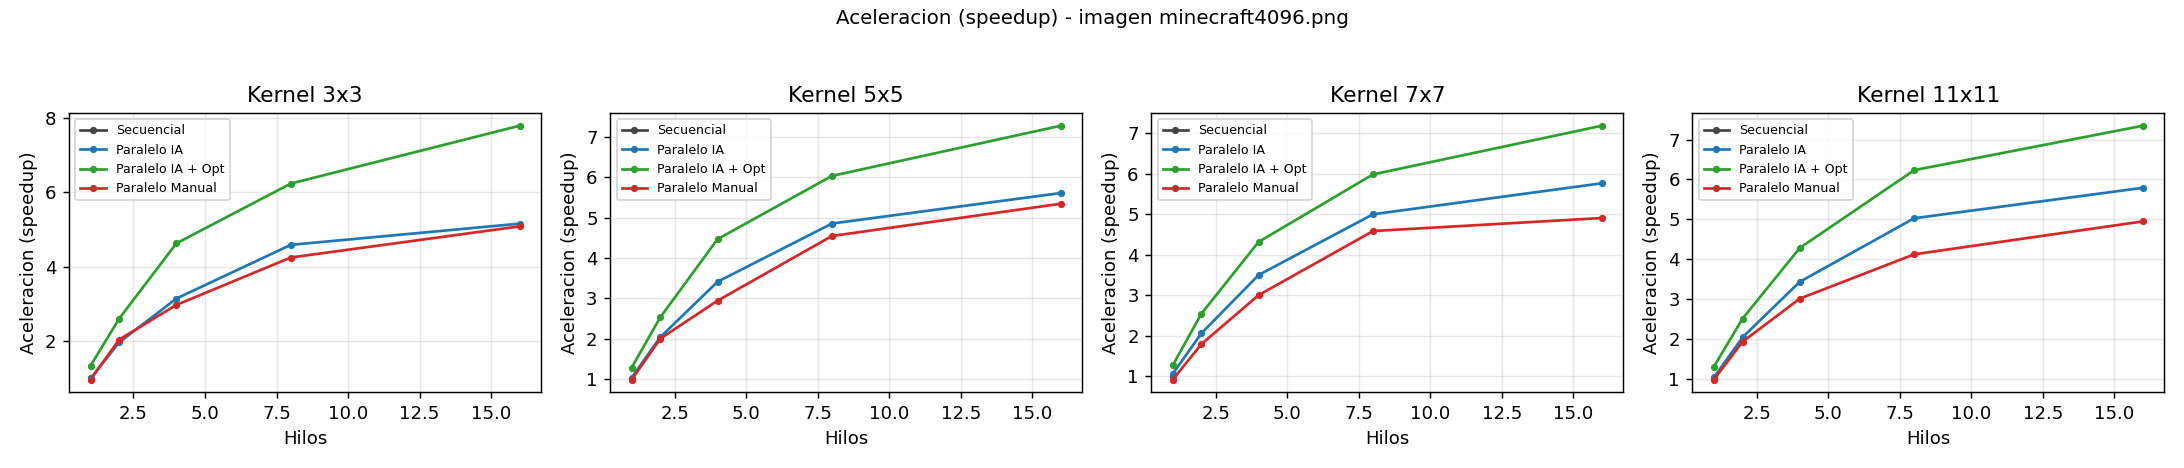
\includegraphics[width=0.9\linewidth]{comparacion_speedup.png}
  \caption{Speedup vs.\ número de hilos: comparación directa entre variantes sobre
  la imagen más grande.}
  \label{fig:speedup}
\end{figure}

\begin{figure}[H]\centering
  \begin{subfigure}[b]{0.32\linewidth}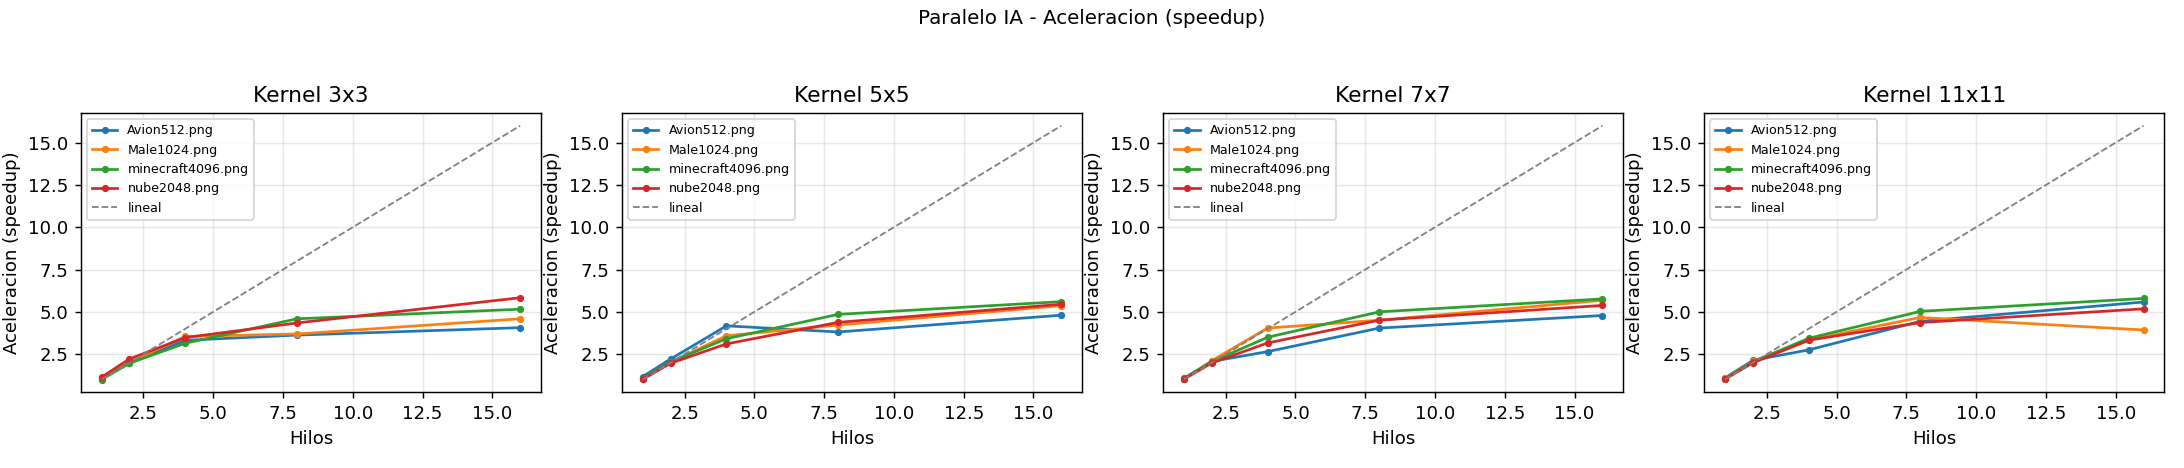
\includegraphics[width=\linewidth]{speedup_paralelo_ia.png}\caption{Paralelo IA}\end{subfigure}
  \hfill
  \begin{subfigure}[b]{0.32\linewidth}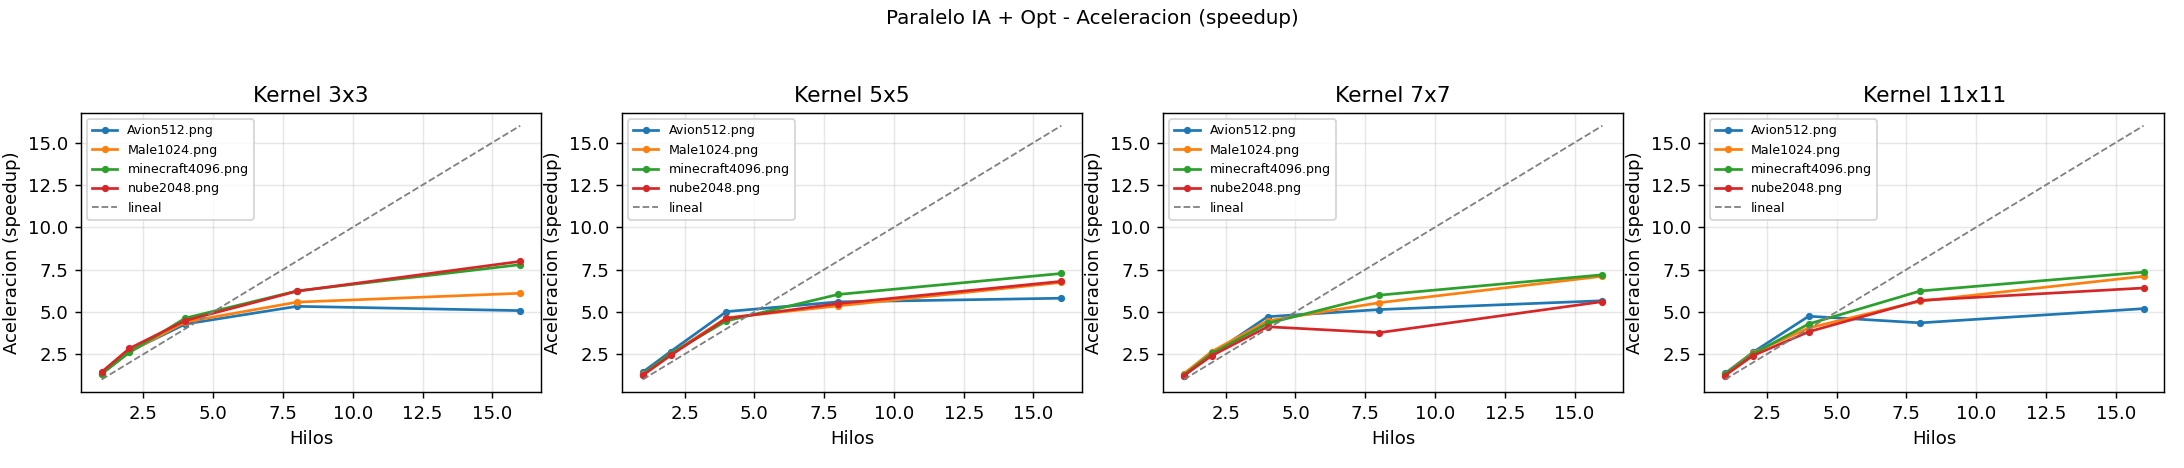
\includegraphics[width=\linewidth]{speedup_paralelo_ia_opt.png}\caption{Paralelo IA~+~Opt}\end{subfigure}
  \hfill
  \begin{subfigure}[b]{0.32\linewidth}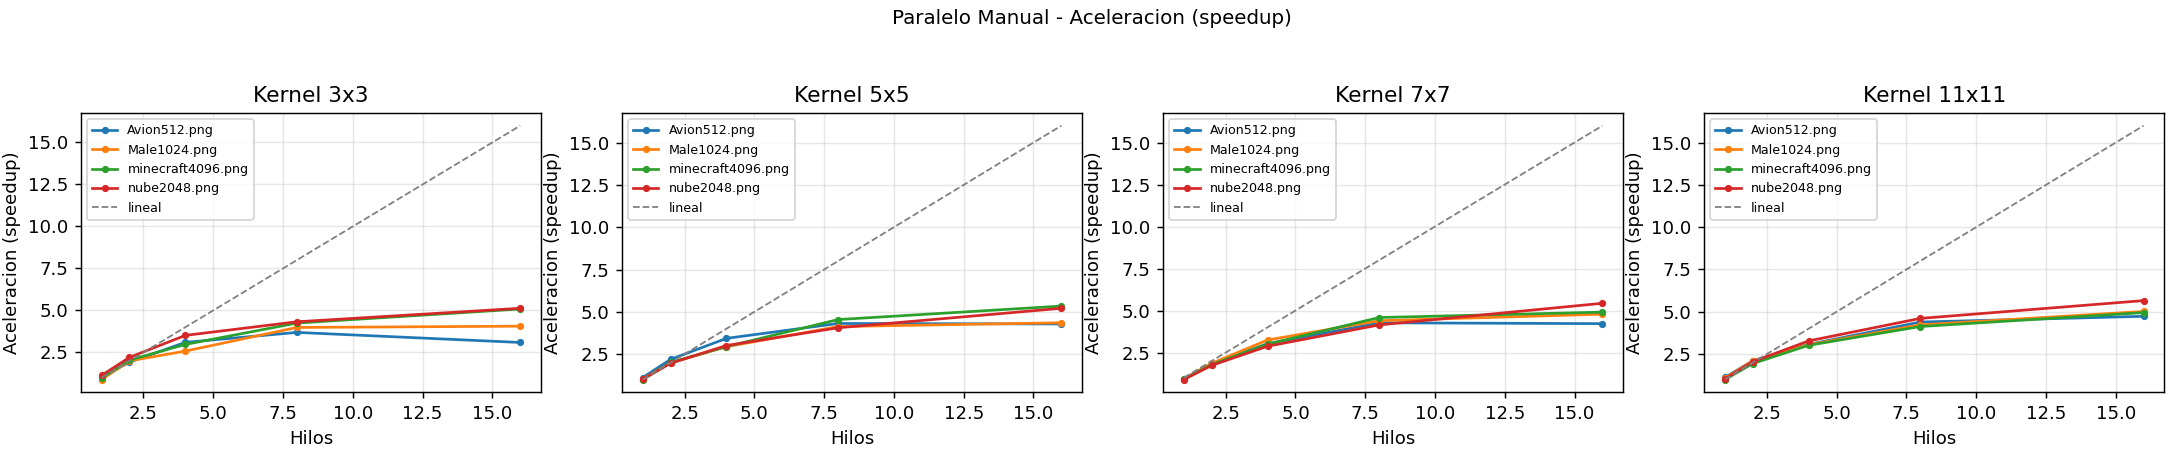
\includegraphics[width=\linewidth]{speedup_paralelo_manual.png}\caption{Paralelo Manual}\end{subfigure}
  \caption{Speedup vs.\ hilos por variante.}
  \label{fig:speedup_prog}
\end{figure}

\subsection{Eficiencia}
La Tabla~\ref{tab:eficiencia} presenta la eficiencia (Ec.~\ref{eq:speedup}).
IA~+~Opt mantiene la mayor eficiencia en todo el rango (0.46 a 16 hilos frente a
0.36 de IA y 0.31 de Manual). La eficiencia cae por debajo de 0.5 a 16 hilos en
las tres variantes y, para IA y Manual, ya a 8 hilos en algunas configuraciones.
Los valores $>1$ a un hilo de IA~+~Opt no indican \emph{superlinealidad} del
paralelismo, sino que la referencia $T_1$ es la versión secuencial sin optimizar.
La Fig.~\ref{fig:eficiencia} desglosa la eficiencia por variante.

\begin{table}[H]
\centering
\caption{Eficiencia $E(p)=S(p)/p$, imagen $4096\times4096$, kernel $11\times11$.}
\label{tab:eficiencia}
\small
\begin{tabular}{@{}lrrrrr@{}}
\toprule
\textbf{Variante} & \textbf{1 h} & \textbf{2 h} & \textbf{4 h} & \textbf{8 h} & \textbf{16 h} \\
\midrule
Paralelo IA        & 1.04 & 1.02 & 0.86 & 0.63 & 0.36 \\
Paralelo IA~+~Opt  & 1.32 & 1.26 & 1.07 & 0.78 & 0.46 \\
Paralelo Manual    & 0.99 & 0.97 & 0.75 & 0.52 & 0.31 \\
\bottomrule
\end{tabular}
\end{table}

\begin{figure}[H]\centering
  \begin{subfigure}[b]{0.32\linewidth}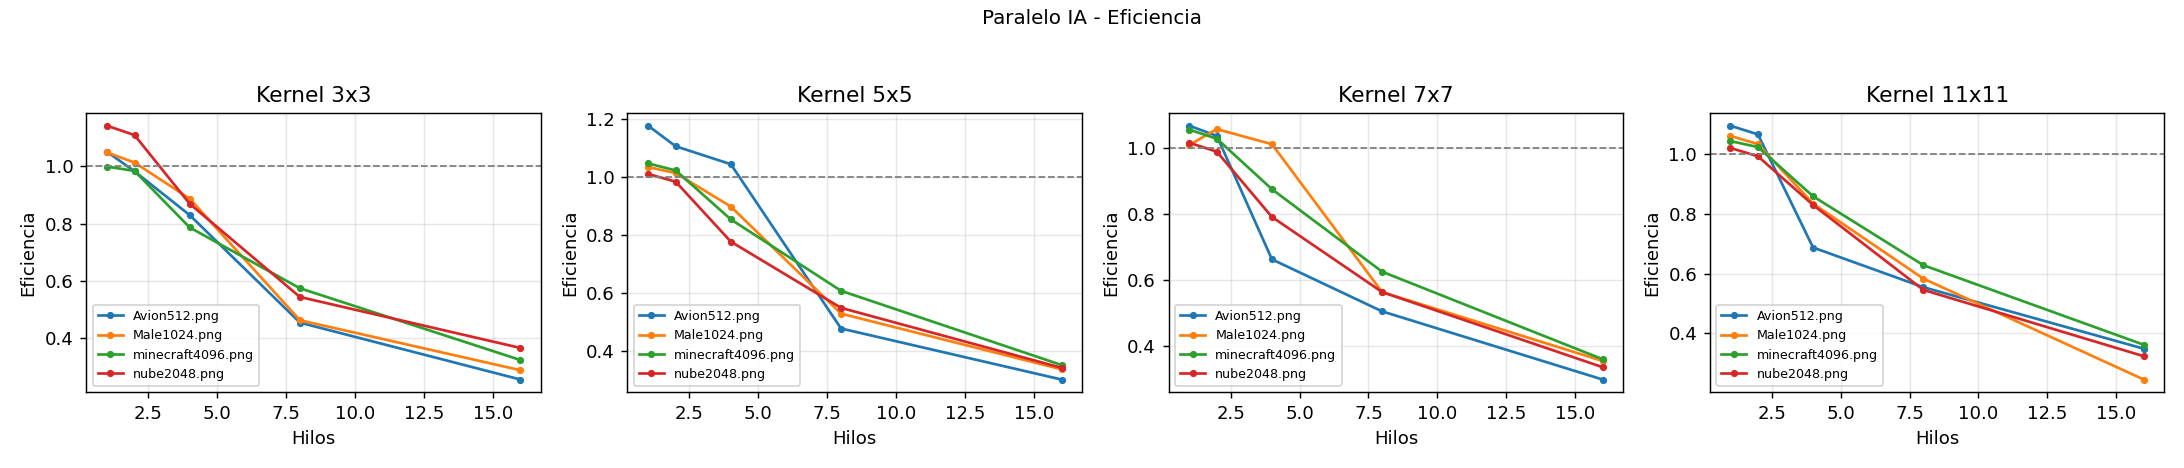
\includegraphics[width=\linewidth]{eficiencia_paralelo_ia.png}\caption{Paralelo IA}\end{subfigure}
  \hfill
  \begin{subfigure}[b]{0.32\linewidth}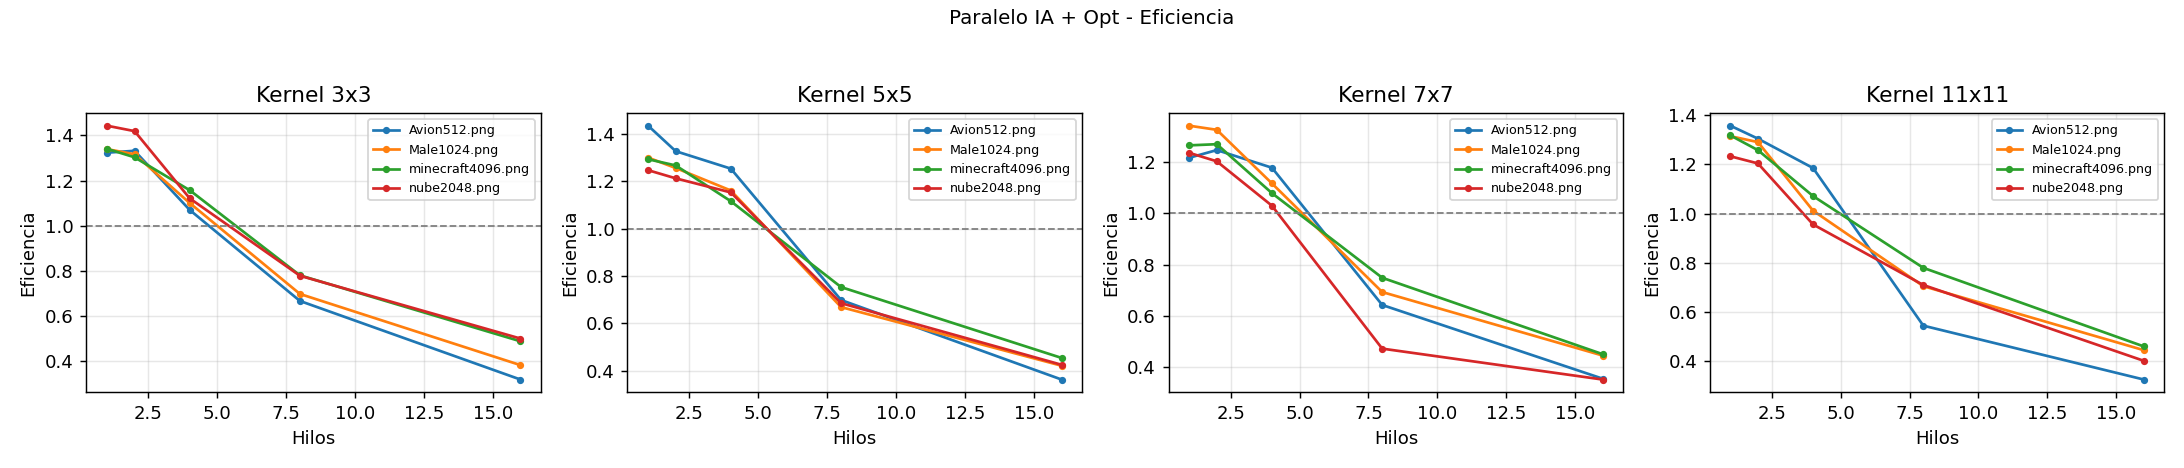
\includegraphics[width=\linewidth]{eficiencia_paralelo_ia_opt.png}\caption{Paralelo IA~+~Opt}\end{subfigure}
  \hfill
  \begin{subfigure}[b]{0.32\linewidth}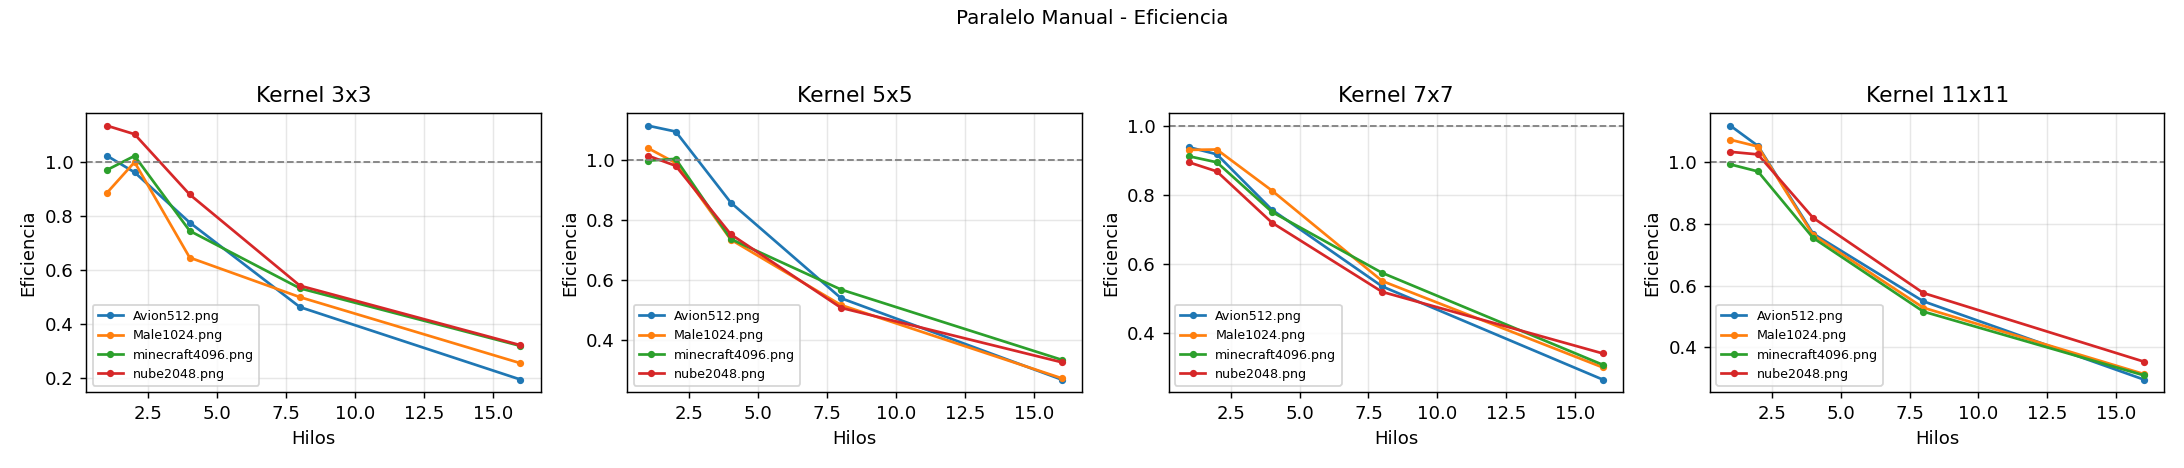
\includegraphics[width=\linewidth]{eficiencia_paralelo_manual.png}\caption{Paralelo Manual}\end{subfigure}
  \caption{Eficiencia vs.\ hilos por variante.}
  \label{fig:eficiencia}
\end{figure}

\subsection{Comparación entre variantes e hipótesis}
\textbf{H1 (IA $\approx$ manual):} se confirma. Ambas variantes alcanzan speedups
similares a 16 hilos en $4096\times4096$ (promedios de $5.58\times$ y $5.07\times$
sobre los cuatro kernels), lo que muestra que el código generado por IA es
competitivo con el escrito a mano para esta carga.

\textbf{H2 (IA~+~Opt $>$ IA a un hilo):} se confirma. A un solo hilo, IA~+~Opt
mejora a IA en un 24.6\,\% en promedio sobre las 16 combinaciones
(imagen$\times$kernel), con un rango de +14.2\,\% a +34.2\,\%. Como este hilo usa el
mismo algoritmo paralelo, la ganancia proviene solo de la reestructuración de
bucles (SIMD) y de la fusión de canales.

\textbf{H3 (eficiencia decreciente):} se confirma. La eficiencia cae
monótonamente con los hilos y a 16 hilos baja de 0.5 en las tres variantes. El
equipo tiene 8 núcleos físicos (4 P + 4 E) y 12 hilos lógicos, de modo que 16
hilos implican \emph{oversubscription}; además, los núcleos E limitan la escalado.

\paragraph{Anomalías.} Se observa un valor atípico en Paralelo IA con la imagen
$1024\times1024$ y kernel $11\times11$ a 16 hilos ($S=3.93$, $E=0.25$), muy por
debajo de la tendencia ($\approx5.4\times$); es consistente con ruido de
planificación en configuraciones dominadas por sincronización.

\subsection{Amenazas a la validez}
\begin{itemize}[leftmargin=1.4em,itemsep=1pt]
  \item \textbf{Validez interna:} los núcleos P/E y el \emph{hiperhilo} introducen
  heterogeneidad; a 16 hilos el \emph{oversubscription} degrada el rendimiento por
  contención de memoria y de ancho de banda. El ruido térmico y de planificación
  infla la desviación estándar en configuraciones cortas (por ejemplo, la
  secuencial $512\times512$ con kernel $3\times3$ tiene $\mu=9.56$ ms y $s=1.18$ ms,
  $\approx12$\,\% de variación).
  \item \textbf{Validez externa:} los resultados corresponden a una única carga,
  un único lenguaje y un único equipo; no se generalizan directamente a otras
  cargas ni a otros entornos.
  \item \textbf{Sobre la IA:} el código generado puede depender del modelo y del
  \emph{prompt} empleados; aquí se documenta el prompt y el origen de cada variante
  (Sección~\ref{sec:metodos}).
\end{itemize}

% ============================================================================
\section{Conclusiones}
\label{sec:conclusiones}

La paralelización del código C++ generado por IA reduce de forma sustancial el
tiempo de convolución: hasta $7.98\times$ en el mejor caso y $7.35\times$ en la
imagen mayor con kernel $11\times11$. El código generado por IA es
\textbf{competitivo} con la implementación escrita a mano (H1: $5.58\times$ frente
a $5.07\times$ a 16 hilos en $4096\times4096$). La optimización posterior
(IA~+~Opt) aporta una mejora clara ya a un hilo (24.6\,\% en promedio) y eleva el
speedup máximo del estudio, confirmando que las ganancias provienen de
reorganizar memoria y aprovechar SIMD, no de paralelizar mejor. La eficiencia cae
por debajo de 0.5 a 16 hilos (3 variantes) por usar más hilos que núcleos físicos
(8 núcleos, 12 hilos lógicos); en la práctica conviene limitar la ejecución a
8--12 hilos. Como trabajo futuro se propone repetir el estudio con
\emph{pinning} de hilos a núcleos P y comparar con otras cargas y otros modelos de
IA.

% ============================================================================
%  Anexo B (revision critica / evaluacion mediante IA) se incorporara aqui
%  cuando este disponible, con:  \input{revision}
%  Ver LEEME.md.

\begin{thebibliography}{9}
\small

\bibitem{githubconv} ivandres73, ``Convolution,'' GitHub repository. [Online].
Available: https://github.com/ivandres73/Convolution.git

\bibitem{stb} S. Barrett, ``stb: single-file public domain libraries for
C/C++,'' GitHub repository. [Online]. Available: https://github.com/nothings/stb

\end{thebibliography}

% ============================================================================
\appendix

\section{Reproducibilidad (comandos)}
\label{anexo:repro}

Los comandos siguientes, ejecutados desde la raíz del proyecto, reproducen el
experimento completo. La suma de comprobación (\emph{checksum}) garantiza que las
cuatro variantes son equivalentes.

\begin{lstlisting}
REM 1) Construir la imagen con las cuatro variantes (una sola vez)
docker build -t benchmark-paralelo .

REM 2) Corrida oficial (30 repeticiones), resultados en resultados/
docker run --rm -v "%cd%\resultados:/resultados" benchmark-paralelo

REM 3) Prueba rapida (3 repeticiones)
docker run --rm -e BENCH_REPS=3 -v "%cd%\resultados:/resultados" benchmark-paralelo
\end{lstlisting}

Artefactos producidos: \texttt{resultados/resultados.csv} (datos crudos),
\texttt{resultados/combinado.csv} (con \texttt{speedup} y \texttt{eficiencia}),
\texttt{resultados/tablas.md} (tablas) y \texttt{resultados/graficas/*.png}
(figuras).

\subsection{Cobertura de lo solicitado en el enunciado}
La Tabla~\ref{tab:cobertura} relaciona cada punto solicitado con la sección (o
tabla/figura) donde se cubre.

\begin{table}[H]
\centering
\caption{Correspondencia con los requisitos del enunciado.}
\label{tab:cobertura}
\small
\begin{tabularx}{\linewidth}{@{}X l@{}}
\toprule
\textbf{Requisito} & \textbf{Se cubre en} \\
\midrule
Objetivo general (impacto de la paralelización en código IA) & Sec.~\ref{sec:intro}, Sec.~\ref{subsec:objetivo} \\
Imágenes $512/1024/2048/4096$ px & Sec.~\ref{subsec:datos} \\
Kernels $3/5/7/11$ & Sec.~\ref{subsec:datos} \\
Escalabilidad de hilos $1/2/4/8/16$ & Sec.~\ref{subsec:protocolo} \\
Validación de equivalencia estricta con la secuencial & Sec.~\ref{subsec:validacion}, Tabla~\ref{tab:validacion} \\
Cuatro variantes (Secuencial, IA, IA+Opt, Manual) & Tabla~\ref{tab:variantes}, Sec.~\ref{subsec:variantes} \\
Manual buscado/adaptado de GitHub, sin usar IA & Sec.~\ref{subsec:variantes} \\
30 ejecuciones por configuración & Sec.~\ref{subsec:protocolo} \\
Medición exclusiva del tiempo de convolución & Sec.~\ref{subsec:protocolo} \\
Métricas (tiempo, speedup, eficiencia) y gráficas & Sec.~\ref{subsec:metricas}, Sec.~\ref{sec:resultados} \\
\bottomrule
\end{tabularx}
\end{table}

\bigskip
\noindent\textbf{Declaración sobre el uso de IA.} La variante ``Paralelo IA'' fue
generada por un asistente de IA; la variante ``Paralelo IA~+~Opt.'' parte de ella y
se optimizó con asistencia de IA; la variante ``Paralelo Manual'' se adaptó de
código humano \cite{githubconv}; el arnés de medición, los \emph{scripts} y las
gráficas se elaboraron con ayuda de IA, bajo revisión de los autores.

\end{document}
